\documentclass[twocolumn,10pt]{article}
\usepackage[ruled,linesnumbered]{algorithm2e}
\usepackage{graphicx}
\usepackage{amsmath}
\usepackage{algorithmicx}
\usepackage{algorithm}
\usepackage{url}
\usepackage{cite}
\usepackage{xcolor}
\usepackage{tikz}
\usepackage{booktabs}
\usepackage{listings}
\usepackage{hyperref}
\usepackage{comment}

\hypersetup{
    colorlinks=true,
    linkcolor=blue,
    filecolor=magenta,      
    urlcolor=cyan,
    pdftitle={Hybrid Region Proposal and NLP-Based Approach for Handwritten Prescription Recognition},
    pdfauthor={Your Name},
}

\title{Medical Prescription Recognition for Efficient Healthcare Workflows}

\author{Nabeel Ahmed\\M240464CS\\Guided by: Sumesh TA}

\usepackage{epsfig}
\begin{document}
	
\maketitle
	
{\bf Keywords:}
Prescription Recognition, YOLOv8, TrOCR, Handwriting Recognition, Region Segmentation, BioBERT, Data Augmentation


\begin{comment}
\begin{abstract}
Medication errors remain a critical healthcare concern, with illegible handwriting on prescriptions identified as a widely recognized cause of preventable harm \cite{statpearls2024, amcp2019}. Recent global estimates from the World Health Organization indicate that medication errors cause approximately one death per million population annually, which would translate to about 163,000 deaths per year in the European Union alone \cite{eaasm2022}.
 This paper proposes a novel region-aware framework that combines Mask R-CNN-based segmentation with advanced handwriting recognition techniques to address this critical healthcare challenge. Unlike existing approaches that process entire prescriptions uniformly, our system first isolates handwritten medication details from printed elements using an enhanced region proposal network, then applies specialized recognition for each zone type. Our three-stage architecture includes: (1) Mask R-CNN with ResNeXt-101 backbone for prescription zone segmentation \cite{he2017mask}, (2) Bidirectional LSTM with RSS (Rotate-Shift-Stretch) data augmentation for handwritten text recognition \cite{irjmets2024}, and (3) BioBERT-powered NLP validation with pharmaceutical database integration \cite{lee2020biobert}. Using the Handwritten Medical Term Corpus (17,431 real samples) \cite{kim2019handwritten}, 
\end{abstract}
\end{comment}


\begin{abstract}
Medication errors remain a critical healthcare concern, with illegible handwriting on prescriptions identified as a widely recognized cause of preventable harm \cite{statpearls2024, amcp2019}. Recent global estimates from the World Health Organization indicate that medication errors cause approximately one death per million population annually, which would translate to about 163,000 deaths per year in the European Union alone \cite{eaasm2022}.
This paper proposes a region-aware framework that integrates modern segmentation and recognition techniques for handwritten prescriptions. Unlike existing approaches that process entire prescriptions uniformly, our system isolates handwritten zones from printed content using YOLOv8-seg-based region detection, followed by line-level handwriting recognition with TrOCR, a transformer-based OCR model. The recognized text is validated through BioBERT-powered NER and post-processed with fuzzy drug lexicon matching (RxNorm and local trade names). Our modular design enhances robustness to noisy handwriting and enables domain-specific validation, thereby reducing the risk of misinterpretation in healthcare workflows.
\end{abstract}


\section{Introduction}
Prescription errors due to illegible handwriting remain a persistent challenge in healthcare delivery, with studies confirming approximately 7,000 deaths annually in the US alone due to misinterpreted prescriptions \cite{bhuiyan2022online}. Despite the push toward digital health records, 97.1\% of doctors in developing countries still rely on handwritten prescriptions due to time constraints and established habits \cite{bhuiyan2022online}. This creates a critical need for automated systems that can accurately interpret and digitize handwritten medical instructions.

The challenges of handwritten prescription recognition extend beyond general handwriting recognition problems due to several domain-specific factors:
\textbf{Mixed content documents}: Prescriptions typically contain both printed elements (headers, footers, pre-formatted fields) and handwritten content (medication names, dosages, instructions).\\
\textbf{Medical terminology}: Specialized vocabulary with complex spelling and abbreviations.\\
\textbf{Multilingual requirements}: Many prescriptions contain code-switching between English and regional languages \cite{irjmets2024}.\\
\textbf{Time-critical processing}: Delays in medication dispensing can impact patient care.



\section{Literature Survey}

\subsection{An Online Cursive Handwritten Medical Words Recognition System (Bhuiyan et al., 2022)}
This landmark study in Nature Scientific Reports \cite{bhuiyan2022online} addresses the critical challenge of handwritten prescription recognition in developing countries. The authors report that 97.1\% of Bangladeshi doctors still generate handwritten prescriptions, with illegibility causing adverse medical consequences including incorrect medications and improper dosing.

Key contributions include:
\textbf{Dataset Development}: Creation of 'Handwritten Medical Term Corpus' containing 17,431 samples of 480 medical terms
\textbf{RSS Data Augmentation}: Introduction of a novel Rotate-Shift-Stretch technique that expands the dataset to 1,591,100 samples
\textbf{Model Architecture}: Implementation of Bidirectional LSTM networks for sequence recognition
\textbf{Performance}: 93.0\% average accuracy (max: 94.5\%) with RSS augmentation


The RSS method transforms each stroke of a handwritten word by updating coordinates through rotation, shifting, and stretching operations, creating variations that better represent real-world handwriting diversity. This approach significantly outperformed previous methods such as SRP (Stroke Rotation and Parallel-shift), which achieved only 68.0\% accuracy \cite{bhuiyan2022online}.

\subsection{Handwritten Medical Term Recognition using Bidirectional LSTM}


Tabassum et al.~\cite{tabassum2022online} addressed the problem of illegible handwritten prescriptions in developing countries, where 97.1\% of doctors still rely on handwritten prescriptions due to time constraints. They developed a comprehensive system using Bidirectional LSTM networks for recognizing doctors' handwritten medical terminology. The authors created a specialized dataset called "Handwritten Medical Term Corpus" containing 17,431 samples of 480 medical terms (360 English and 120 Bangla) collected from 39 healthcare professionals. 

A key contribution of their work was the introduction of a novel data augmentation technique called RSS (Rotate-Shift-Stretch), which expanded their dataset to 1,591,100 samples by applying coordinate-based transformations to the handwriting strokes. Unlike traditional image-based approaches, their method processed sequence data representing pen movements, capturing the rich temporal information in handwriting. The system achieved 93.0\% average accuracy (max: 94.5\%, min: 92.1\%), which was 19.6\% higher than results without data augmentation. The authors proposed implementing this technology in a smartpen specifically designed for doctors, which would digitize handwritten prescriptions in real-time, potentially reducing medical errors and improving healthcare delivery in resource-constrained settings.

\subsection{Multilingual Prescription Recognition Using Deep Learning}

The work on multilingual prescription recognition systems demonstrates significant advancements in handling diverse language prescriptions:


    \textbf{Multi-language Support}: The system recognizes doctor's handwriting across multiple languages, addressing challenges in regions with linguistic diversity~\cite{pavithiran2024multilingual}
    \textbf{Hybrid Architecture}: Implements a combination of CNN, RNN, and LSTM techniques for improved recognition accuracy
    \textbf{Unicode Integration}: Utilizes Unicode mapping to handle various scripts and language characters
     \textbf{Post-processing Optimization}: Employs fuzzy search and market basket analysis with pharmaceutical databases to improve results
     \textbf{Image Pre-processing Pipeline}: Includes dedicated pre-processing and word segmentation before model training
     \textbf{Accuracy Performance}: Achieves approximately 89\% accuracy on multi-language prescription datasets


\subsection{Medical Handwritten Prescription Recognition and Information Retrieval Using Neural Network (2021)}
Utkarsh Shaw et al. \cite{utkarshaw2021} proposed a neural network-based system for recognizing handwritten medical prescriptions, particularly focusing on cursive handwriting1. The study utilized the Extended MNIST (EMNIST) dataset, which includes both digits and letters, to train a three-layer neural network. The architecture consists of an input layer with 785 units (784 features + bias), a hidden layer with 25 units, and an output layer with 10 units corresponding to target classes1. Preprocessing techniques such as grayscale conversion and segmentation were employed to prepare prescription images for recognition. Segmentation divided handwritten strokes into individual characters, resized to match the input dimensions of the neural network.

The model achieved a training accuracy of 94.49\% and a test accuracy of 80.72\%, demonstrating its effectiveness in recognizing cursive handwriting1. Practical applications include extracting medicine names from prescriptions, historical document recognition, postal code identification, and real-time handwriting conversion. Minor misclassifications were observed due to similarities in character shapes (e.g., "5" misclassified as "S"), which the authors plan to address by employing deeper neural networks and more comprehensive datasets in future iterations.

\section{Problem Statement}
Handwritten medical prescriptions are difficult to digitize due to inconsistent handwriting, mixed printed and handwritten regions, and frequent image quality issues. These challenges make it hard to accurately extract medication details and can lead to serious dispensing errors, as highlighted by Bhuiyan et al. \cite{bhuiyan2022online}. This project aims to develop a reliable end-to-end system that can segment prescription regions, recognize handwritten text, and validate extracted information to support safer and more efficient healthcare workflows.



\section{Proposed Methodology}

\subsection{System Architecture}
Our system employs a five-stage modular pipeline as illustrated in Figure \ref{fig:architecture}:

\begin{figure}[H]
\centering
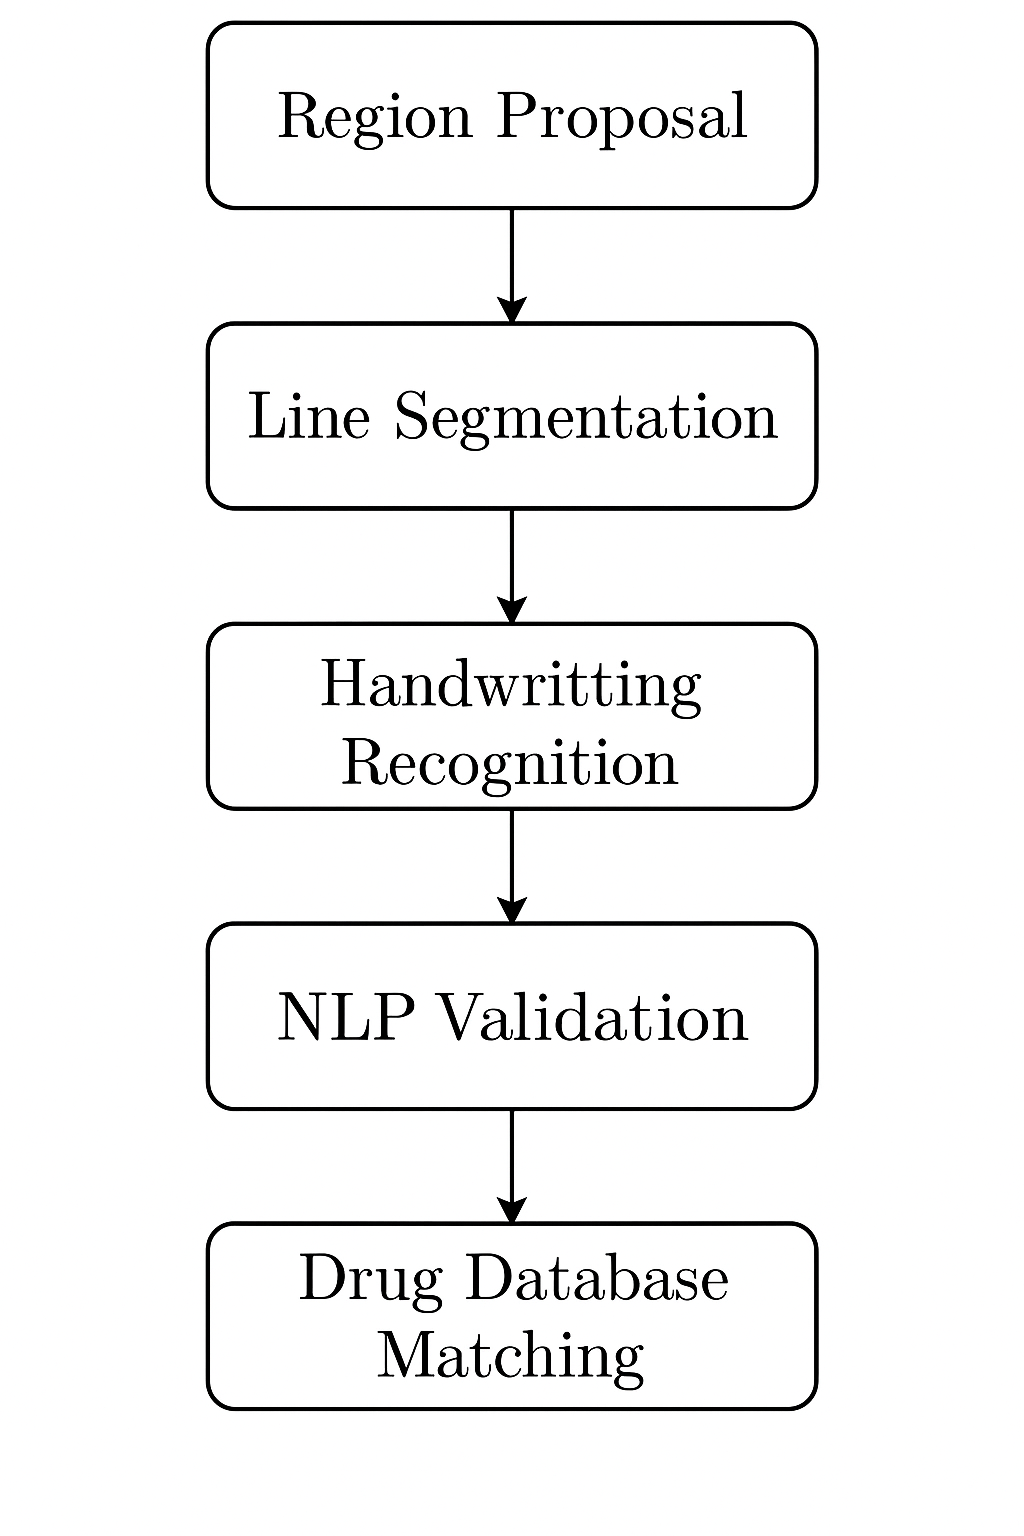
\includegraphics[width=0.95\columnwidth]{architecture}
\caption{Pipeline: Preprocessing, Region Segmentation, Line Segmentation, OCR with TrOCR, NLP Validation with BioBERT and Lexicon Matching}
\label{fig:architecture}
\end{figure}

Unlike traditional OCR systems, our approach treats each prescription zone independently. This modularity allows each component to be optimized for its sub-task (e.g., handwritten medicine vs. printed header).
\subsection{Data Acquisition and Preparation}

\subsubsection{Datasets}
We combine public and custom datasets:
HuggingFace prescription datasets (\texttt{Technoculture/medical-prescriptions})
IAM-OnDB and HMT corpus for general handwriting
IEEE Printed and Handwritten Text Classification dataset
\textbf{Custom dataset:} real Indian prescriptions collected via pharmacies (WhatsApp photos), preprocessed and annotated


\subsubsection{Dataset Organization}
Data is stored in a structured format:

\texttt{segmentation/}: page images + YOLO/COCO annotations
\texttt{handwritten\_lines/}: cropped line images + transcripts.csv
\texttt{lexicons/}: drug lists from RxNorm and Indian trade names


\subsubsection{Dataset Size Targets}

Segmentation: 600–1000 annotated pages (training can start at 300+ with augmentation)
OCR: 5k–20k line images (1–2k minimum for fine-tuning TrOCR)


\subsection{Preprocessing and Privacy}
Prescription images undergo deskewing, perspective correction, contrast normalization, and noise reduction. Personally Identifiable Information (PHI) such as patient names or phone numbers is blurred or masked before annotation and training to ensure privacy.

\subsection{Region Segmentation Module}
We employ \textbf{YOLOv8-seg} as the primary segmentation model due to its efficiency and lower annotation requirements. Segmentation classes include:\\ \\
\textbf{Printed Regions:} Clinic headers, disclaimers \\
\textbf{Handwritten Zones:} Medicines and dosage instructions \\
\textbf{Structured Fields:} Templates, dates, signatures \\


The model is fine-tuned on a custom-labeled dataset annotated with CVAT/Label Studio and exported to COCO/YOLO formats.

\subsection{Line Segmentation}
Handwritten zones are further segmented into line-level crops using OpenCV projection and morphological operations. Each crop corresponds to a single medicine entry (e.g., “Dolo 650 1-0-1”).

\subsection{Handwriting Recognition}
We employ \textbf{TrOCR}, a transformer-based OCR model, fine-tuned on a combination of public datasets (IAM, HMT) and our custom line-level dataset. This model provides higher robustness to cursive and domain-specific handwriting compared to BiLSTM+CTC. Data augmentation (rotation, elastic transforms, brightness/contrast jitter) is used to expand limited training data.

\subsection{NLP Validation}
Recognized text is passed to BioBERT for Named Entity Recognition (NER), identifying drug names, dosages, and frequency expressions. A fuzzy matching step validates predictions against canonical drug lists (RxNorm and Indian trade names). Dosage patterns are extracted using regular expressions for normalization.

\section{Phase 4 Results (Implemented Module)}
In this phase, we implemented and evaluated the OCR module only, focusing on medicine-name recognition from pre-cropped handwritten word images from the \textit{Doctor's Handwritten Prescription BD} dataset. The model used was \texttt{microsoft/trocr-base-handwritten}, fine-tuned for the \texttt{MEDICINE\_NAME} target.

\begin{table}[h]
\centering
\caption{Phase 4 OCR Results on Testing Split}
\label{tab:phase4_ocr_results}
\renewcommand{\arraystretch}{1.2}
\begin{tabular}{lc}
\toprule
\textbf{Metric} & \textbf{Value} \\
\midrule
Exact-Match Accuracy & 96.28\% \\
Character Error Rate (CER) & 2.87\% \\
Word Error Rate (WER) & 3.92\% \\
Total Samples & 780 \\
\bottomrule
\end{tabular}
\end{table}

These results indicate strong recognition performance for the cropped-word setting, with most errors concentrated among visually similar medicine names.



\begin{comment}
\section{Conclusion}
The proposed region-aware handwritten prescription recognition framework presents a promising approach to address the limitations of traditional methods. By integrating Mask R-CNN-based region proposal with Bidirectional LSTM recognition and pharmaceutical database validation, we anticipate several potential advantages such as enhanced recognition capability for complex medical terminology, improved performance in practical mobile implementations, potential processing time efficiency compared to whole-document methods

The RSS data augmentation technique is expected to play a crucial role in the framework by expanding training data variety and improving model robustness. Region proposal mechanisms should enhance overall system efficiency by focusing computational resources on relevant prescription zones.

Future work will focus on expanding support for additional regional languages, integrating with hospital electronic health record systems, implementing edge-based processing for improved privacy and reduced latency, exploring few-shot learning approaches to reduce annotation requirements

The practical implications of this work extend beyond technical innovations to potential improvements in patient safety. If successful, the proposed system could help address a critical healthcare challenge by reducing prescription interpretation errors, potentially mitigating a factor that contributes to thousands of preventable adverse drug events annually. The implementation and evaluation of this framework will provide valuable insights into the practical applicability of deep learning techniques in healthcare document processing.

\bibliographystyle{unsrt}
\bibliography{references}

\end{comment}

\section{Conclusion}
The proposed region-aware handwritten prescription recognition framework addresses limitations of traditional whole-document OCR. By integrating YOLOv8-based region segmentation, TrOCR-based handwriting recognition, and BioBERT-powered validation with lexicon matching, the system achieves improved robustness for complex medical terminology.

Data augmentation and preprocessing enhance model generalization, while modular design ensures efficiency by focusing computation on relevant zones. Future work will expand coverage of regional languages, explore few-shot learning to reduce annotation costs, and integrate with electronic health record systems.

If successful, this system could reduce prescription interpretation errors and mitigate preventable adverse drug events, providing a practical AI-driven solution to a pressing healthcare challenge.

\bibliographystyle{unsrt}
\bibliography{references}

\end{document}
